\section{Design patterns}
Tijdens het realiseren van de afstudeer opdracht is er gebruik gemaakt van het Repository pattern.
Dit pattern en een \textbf{ander pattern wat ik nog moet verzinnen} zijn beschreven in de volgende delen.

\subsection{Repository pattern}
Het repository pattern is een structural design pattern wat de data en logica van de applicatie schied.
Dit wordt gedaan door middel van een abstracte tussen laag waarmee de logica en de data laag mee communiceren.

\whitespace
Hierdoor wordt de logica en de data van elkaar gescheiden en wort er voldaan aan het single-reponsability principle.
Dit zorgt voor beter testbare code waar door de betrouwbaarheid van het programma om hoog gaat.
Verder zorgt het er voor dat je code base niet vast zit aan één database provider.

\whitespace
Dit is geimplementeerd door de logica af te laten hangen van een interface inplaats van een concrete implementatie.
Een visualisatie van de geimplementeerde versie is te zien in figuur \ref{fig:RepositoryPattern}

\whitespace[2]
\begin{graphic}
    \captionsetup{type=figure}
    \caption{Visualisatie van fields}
    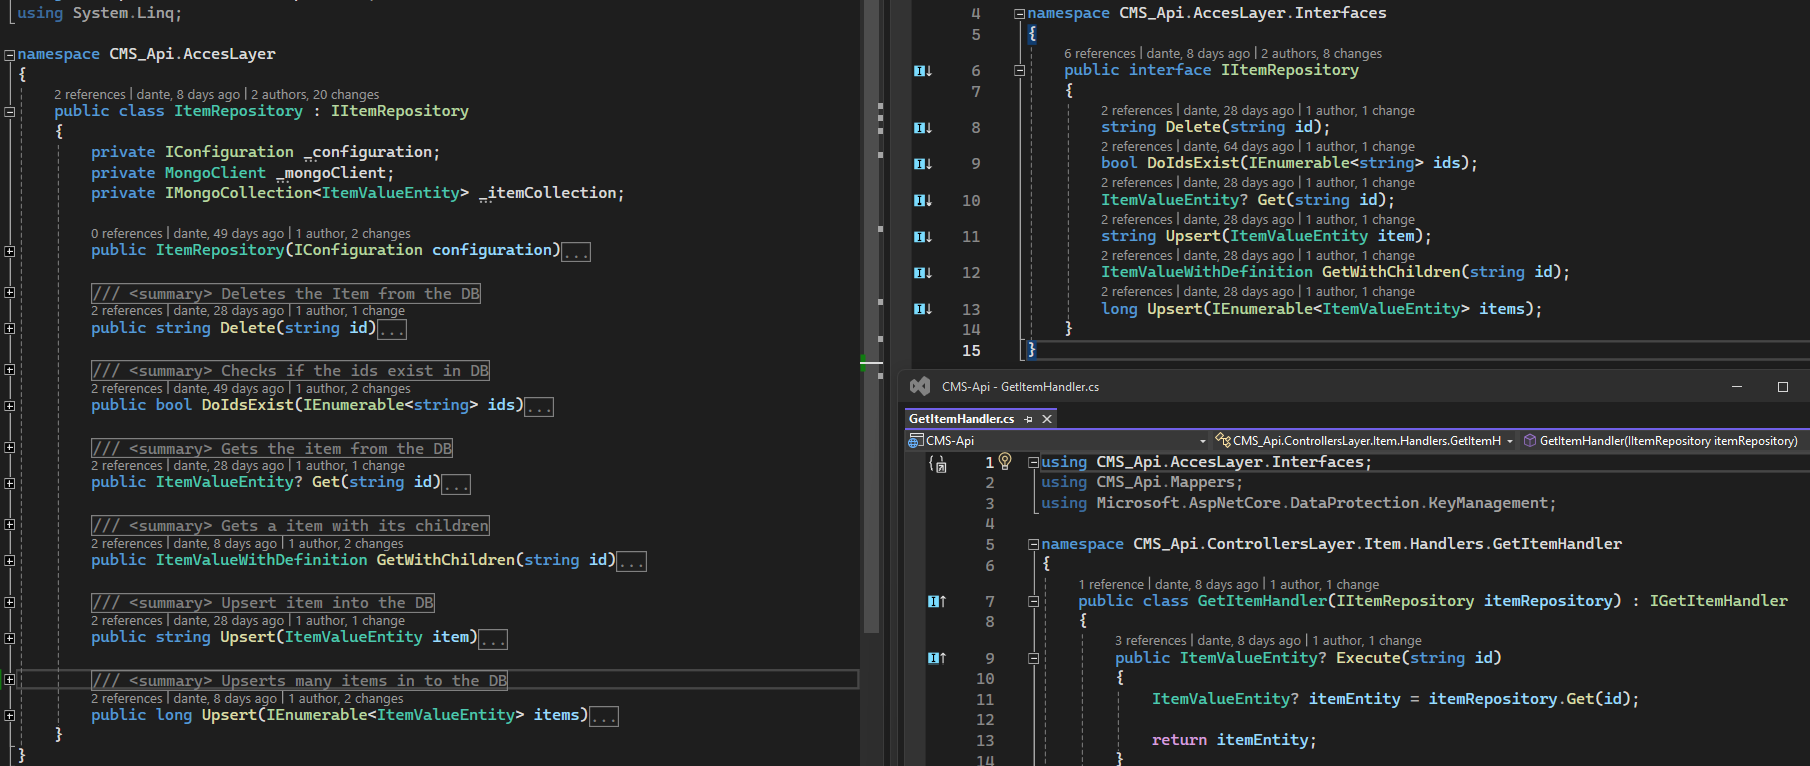
\includegraphics[scale=0.35]{ImplementationRepositoryPattern.png}
    \label{fig:RepositoryPattern}
\end{graphic}
% Het repository pattern is een structural design pattern dat gebruikt wordt om je logica en data \textit{retrieval} te scheiden.
% Door de datalaag te schieden van de logica moet het makkelijker worden om nieuwe databases of andere data storage methodes te implementeren.


